\documentclass[12pt,a4paper,oneside]{report}             % Single-side
%\documentclass[11pt,a4paper,twoside,openright]{report}  % Duplex
%\PassOptionsToPackage{chapternumber=Huordinal}{magyar.ldf}
\usepackage{t1enc}
\usepackage[utf8]{inputenc} % modified from latin2
\usepackage{amsmath}
\usepackage{amssymb}
\usepackage{enumerate}
\usepackage{ntheorem} % [thmmarks] ELRONTJA a \ref-et
\usepackage{graphics}
\usepackage{epsfig}
\usepackage{listings}
\usepackage{color}
%\usepackage{fancyhdr}
\usepackage{lastpage}
\usepackage{anysize}
\usepackage[magyar]{babel}
\usepackage{sectsty}
\usepackage{setspace}  % Ettol a tablazatok, abrak, labjegyzetek maradnak 1-es sorkozzel!
\usepackage[hang]{caption}
\usepackage{hyperref}



%--------------------------------------------------------------------------------------
% EXTRA A SABLONON FELÜL
%--------------------------------------------------------------------------------------
%different font
%\renewcommand{\familydefault}{\sfdefault}



\frenchspacing
\usepackage[T1]{fontenc}
\usepackage{ragged2e}
\usepackage{graphicx}
\usepackage{float}

\usepackage{array}
\usepackage{subcaption} % subfigure
\usepackage{enumitem}
\usepackage{enumitem}
\usepackage{dirtytalk} %say
\usepackage{ntheorem} % cruical to have it WHITOUT [thmmarks] or dont have it all because it will ruin \REF

\usepackage{siunitx}
\usepackage{amsmath}
\usepackage{amssymb}

\usepackage{listings}

\usepackage{titlesec}

%tables
\usepackage{tabu}
\usepackage{tabulary}
\usepackage{multirow} % join cells
\usepackage{makecell} % multiple row
\usepackage{hhline}


% TIKZPICTURES:
\usepackage{pgf}
\usepackage{tikz}
\usepackage{verbatim}
% for the tikz
\usetikzlibrary{shapes,arrows}
\usetikzlibrary{arrows,automata}
\usetikzlibrary{positioning}
\usetikzlibrary{calc}
%\tikzset{anchor/.append code=\let\tikz@auto@anchor\relax} %no auto anchor


\tikzset{
	state/.style={
		rectangle,
		rounded corners,
		draw=black, very thick,
		minimum height=2em,
		inner sep=2pt,
		text centered,
	},
}

%megjegyzésekhez: - nem official
\usepackage{framed} % for defining framed environment
\newenvironment{formal}{
	\def\FrameCommand{{\hspace{18pt}\color{gray}\vrule width 2pt}\hspace{18pt}}
	\MakeFramed{\advance\hsize-\width}
	\vspace{2pt}\noindent\hspace{2pt}\vspace{3pt}
}{\vspace{3pt}\endMakeFramed}


%--------------------------------------------------------------------------------------
% Main variables
%--------------------------------------------------------------------------------------
\newcommand{\vikszerzo}{Gyulai László}
\newcommand{\vikkonzulens}{dr. Kiss Bálint}
\newcommand{\kulsokonzulens}{Kurbucz Máté}
\newcommand{\viktitle}{Modell prediktív fűtésszabályozás\\[12pt] alkalmazási lehetőségei}
\newcommand{\vikcim}{Modell prediktív fűtésszabályozás alkalmazási lehetőségei}
\newcommand{\vikcimBlank}{Korszerű fűtési rendszerek szabályozása}
\newcommand{\viktanszek}{Irányítástechnika és Informatika Tanszék}

\newcommand{\vikdoktipus}{Önálló laboratórium}
\newcommand{\vikmunkatipusat}{szakdolgozatot} % a "hallgató nyilatkozat" részhez: szakdolgozatot vagy diplomatervet

%--------------------------------------------------------------------------------------
% Page layout setup
%--------------------------------------------------------------------------------------
% we need to redefine the pagestyle plain
% another possibility is to use the body of this command without \fancypagestyle
% and use \pagestyle{fancy} but in that case the special pages
% (like the ToC, the References, and the Chapter pages)remain in plane style

\pagestyle{plain} % ellentmond a pagestyle fancy-nek
\setlength{\parindent}{0pt} % áttekinthetőbb, angol nyelvű dokumentumokban jellemző
\setlength{\parskip}{9pt plus 3pt minus 3pt} % áttekinthetőbb, angol nyelvű dokumentumokban jellemző
%\setlength{\parindent}{12pt} % magyar nyelvű dokumentumokban jellemző
%\setlength{\parskip}{0pt}    % magyar nyelvű dokumentumokban jellemző

%\marginsize{35mm}{25mm}{15mm}{15mm} % anysize package
%\marginsize{30mm}{20mm}{12mm}{12mm} % anysize package
\marginsize{35mm}{25mm}{15mm}{15mm} % anysize package - VÉGLEGESHEZ

%\setcounter{secnumdepth}{0}
%\sectionfont{\large\upshape\bfseries}
%\setcounter{secnumdepth}{3}
\singlespacing
\frenchspacing

%--------------------------------------------------------------------------------------
%	Setup hyperref package
%--------------------------------------------------------------------------------------
\hypersetup{
	bookmarks=true,            % show bookmarks bar?
%	unicode=false,             % non-Latin characters in Acrobat�s bookmarks   https://tex.stackexchange.com/questions/53135/glyph-not-defined-in-pd1-encoding-removing-h
 	pdftitle={\vikcim},        % title
	pdfauthor={\vikszerzo},    % author
	pdfsubject={\vikdoktipus}, % subject of the document
	pdfcreator={\vikszerzo},   % creator of the document
	pdfproducer={Producer},    % producer of the document
	pdfkeywords={keywords},    % list of keywords
	pdfnewwindow=true,         % links in new window
	colorlinks=true,           % false: boxed links; true: colored links
	linkcolor=black,           % color of internal links
	citecolor=black,           % color of links to bibliography
	filecolor=black,           % color of file links
	urlcolor=black             % color of external links
}

%--------------------------------------------------------------------------------------
% Set up listings
%--------------------------------------------------------------------------------------
\lstset{
	basicstyle=\scriptsize\ttfamily, % print whole listing small
	keywordstyle=\color{black}\bfseries\underbar, % underlined bold black keywords
	identifierstyle=, 					% nothing happens
	commentstyle=\color{white}, % white comments
	stringstyle=\scriptsize\sffamily, 			% typewriter type for strings
	showstringspaces=false,     % no special string spaces
	aboveskip=3pt,
	belowskip=3pt,
	columns=fixed,
	backgroundcolor=\color{lightgray},
} 		
\def\lstlistingname{lista}	

%--------------------------------------------------------------------------------------
%	Some new commands and declarations
%--------------------------------------------------------------------------------------
%\newcommand{\code}[1]{{\upshape\ttfamily\scriptsize\indent #1}}

% define references
\newcommand{\figref}[1]{\ref{fig:#1}.}
\renewcommand{\eqref}[1]{(\ref{eq:#1})}
\newcommand{\listref}[1]{\ref{listing:#1}.}
\newcommand{\sectref}[1]{\ref{sect:#1}}
\newcommand{\tabref}[1]{\ref{tab:#1}.}

%\DeclareMathOperator*{\argmax}{arg\,max}
%\DeclareMathOperator*[1]{\floor}{arg\,max}
%\DeclareMathOperator{\sign}{sgn}
%\DeclareMathOperator{\rot}{rot}
%\definecolor{lightgray}{rgb}{0.95,0.95,0.95}

\author{\vikszerzo}
\title{\viktitle}

%--------------------------------------------------------------------------------------
%	Setup captions
%--------------------------------------------------------------------------------------
\captionsetup[figure]{
%labelsep={:~},
font={footnotesize,it},
justification=justified,
width=.75\textwidth,
aboveskip=10pt}

% MODIFIED: FOR SUBCAPTIONS
\captionsetup[sub]{
	%labelsep=none,
	labelfont+={footnotesize},
	font={footnotesize,it},
	justification=justified,
	width=.75\textwidth,
	aboveskip=10pt
}

\renewcommand{\captionlabelfont}{\small\bf}
\renewcommand{\captionfont}{\footnotesize\it}



%--------------------------------------------------------------------------------------
% Table of contents and the main text
%--------------------------------------------------------------------------------------
\begin{document}
\pagenumbering{gobble}
\singlespacing
\begin{titlepage}
	\begin{center}
		
\includegraphics[width=60mm,keepaspectratio]{figures/BMElogo.png}\\
		\vspace{0.3cm}
		\textbf{Budapesti Műszaki és Gazdaságtudományi Egyetem}\\
		\textmd{Villamosmérnöki és Informatikai Kar}\\
		\textmd{\viktanszek}\\[1cm]
		\vspace{0.3cm}
				%\includegraphics[width=60mm,keepaspectratio]{figures/SZTAKI.png}\\
					% trim={<left> <lower> <right> <upper>}
		
\includegraphics[width=60mm,keepaspectratio, trim=0 90 0 90, clip,]{figures/icontrall-logo.png}\\
		\vspace{0.3cm}
		\textbf{iContrALL Intelligens Épületelektronika Kft.}\\[5cm]
		
		\vspace{0.4cm}
		{\huge \bfseries \viktitle}\\[0.8cm]
		\vspace{0.5cm}
		\textsc{\Large \vikdoktipus}\\[4cm]
		
		\begin{tabular}{cc}
			\makebox[5cm]{\emph{Készítette}}  \makebox[5cm]{\emph{Belső konzulens}} & \makebox[5cm]{\emph{Külső konzulens}} \\
			 \makebox[5cm]{\vikszerzo} \makebox[5cm]{\vikkonzulens}& \makebox[5cm]{\kulsokonzulens}
		\end{tabular}
		
		\vfill
		{\large \today}
	\end{center}
\end{titlepage}

\bigskip
\bigskip
\tableofcontents
\newpage
%\selectlanguage{magyar}
\pagenumbering{gobble}
%--------------------------------------------------------------------------------------
% Nyilatkozat
%--------------------------------------------------------------------------------------
\begin{center}
\large
\textbf{HALLGATÓI NYILATKOZAT}\\
\end{center}

Alulírott \emph{\vikszerzo}, szigorló hallgató kijelentem, hogy ezt a \vikmunkatipusat{} meg nem engedett segítség nélkül, saját magam készítettem, csak a megadott forrásokat (szakirodalom, eszközök stb.) használtam fel. Minden olyan részt, melyet szó szerint, vagy azonos értelemben, de átfogalmazva más forrásból átvettem, egyértelműen, a forrás megadásával megjelöltem.

Hozzájárulok, hogy a jelen munkám alapadatait (szerző(k), cím, angol és magyar nyelvű tartalmi kivonat, készítés éve, konzulens(ek) neve) a BME VIK nyilvánosan hozzáférhető elektronikus formában, a munka teljes szövegét pedig az egyetem belső hálózatán keresztül (vagy autentikált felhasználók számára) közzétegye. Kijelentem, hogy a benyújtott munka és annak elektronikus verziója megegyezik. Dékáni engedéllyel titkosított diplomatervek esetén a dolgozat szövege csak 3 év eltelte után válik hozzáférhetővé.

\begin{flushleft}
\vspace*{1cm}
Budapest, \today
\end{flushleft}

\begin{flushright}
 \vspace*{1cm}
 \makebox[7cm]{\rule{6cm}{.4pt}}\\
 \makebox[7cm]{\emph{\vikszerzo}}\\
 \makebox[7cm]{hallgató}
\end{flushright}
\thispagestyle{empty}

\vfill
\clearpage
\thispagestyle{empty} % an empty page

%\selectthesislanguage



\pagenumbering{arabic}
\onehalfspacing


\chapter{Szabályzó kiválasztása és analízise}\label{chap:control}

A fejezetben a Simulinkben átviteli függvényre megtervezem a szabályozást. A szabályzó választásakor világossá vált, hogy egy egyszerű PID típusú szabályozás nem képes a rendszert jól kezelni. Igaz, hogy a PID közismert és az iparban egyszerűsége miatt széles körben használt, de épületgépészeti alkalmazásnál egy szabályozás jóságát többféleképp is értelmezhetjük\footnote{Mást tekintünk jó szabályozásnak egy tisztatérben, egy irodában, vagy egy nagyelőadóban, hiszen mások a felmerülő igények, és így a kritériumok is.}. Egyes esetekben hibahatárt megszabva lazíthatunk például a referenciakövetési feltételeken.

Az identifikált modellre többféle szabályzót tervezek, illetve próbálok ki.

A hasonló feladatokra leggyakrabban modell-prediktív (MPC) szabályozást használnak \cite{AFRAM2014343}. Ehhez szükség van a szakasz modelljére, ami alapján a szabályzó szimulálhatja a szakasz kimenetét. Az MPC egy beavatkozójel kiadása előtt több mintavételi perióduson, egy predikciós horizonton keresztül fut le, minden lehetséges  beavatkozójel-sorozatra a kimenetet szimulálva.
%A csúszóablak miatt receding horizon control
Ezen sorozatok közül a legjobbat kiválasztja és egy lépést végrehajt. Ezután a szimuláció újrakezdődik. A végrehajtott, adott horizonton optimális beavatkozójelet egy költségfüggvény minimalizálásával kapja. A költségfüggvényben különböző eltéréseknek vagy abszolútértékeknek különböző súlya lehet.

A szabályozás tehát képes egy horizontig előre tekinteni, és azon belüli optimális beavatkozást végrehajtani. (Az angol nyelvű irodalom erre \textit{receding horizon} névvel hivatkozik.) Az optimalizációt minden mintavételkor végrehajtja, így képes korrigálni, ha a jósolt kimenet és a tényleges kimenet eltérő.

A zárt szabályozási körben a stabilitás viszont nem garantált, erre külön módszerek léteznek (úgynevezett \textit{terminal cost}, azaz végső költség, illetve időben változó súlyozás). Mivel a vizsgált rendszerem nyílt körben is stabil, ezekkel nem kell foglalkoznom.

A stabilitás a beavatkozó jelek és a zavarjel (külső hőmérséklet) korlátosságából fakad. Ezeket is be lehet állítani a szabályzón, így az MPC a szelepekre csak 0 és 1 közötti beavatkozó jelet fog kiadni. A változások hatásait is figyelembe vehetjük, mivel a szelepeket 4-5 perc teljesen kinyitni.

A helyiség hőmérséklet-szabályozásakor a legfontosabb feladat a költségfüggvény súlyainak helyes beállítása\footnote{A súlyozást kiegészíthetik a fizikai korlátok is. Ha a szelepek nyitási- és zárási sebessége korlátos, akkor ezt nem lehet túllépni alacsony súly használatával sem.}. Ezek ugyanis befolyásolják a referenciakövetést - az állandósult állapotbeli hibát és lengést - és a beavatkozójel nagyságát, frekvenciáját is.

Az épületgépészeti rendszereknél a nagyobb frekvenciájú beavatkozójel könnyedén jelenthet alacsonyabb hatásfokot. Viszont ha megengedünk valamennyi ingadozást állandósult állapot körül, a terhelést kiegyenlíthetjük.
Egy irodában, vagy lakásban  például 0.1\si{\celsius}-os vagy 1\si{\celsius}-os pontosságú hőmérséklet-szabályozás közötti különbség komfortban aligha érezhető.
\vspace{6pt}

\begin{figure}[h]
	\centering
	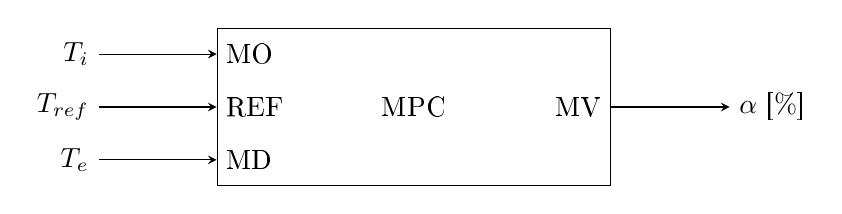
\begin{tikzpicture}[>=stealth]
	% Controller
	% ----------
	\node[draw,rectangle, minimum height=2cm,minimum width=5cm,
		  %label={[xshift=1.0cm, yshift=0.3cm]Label},
		  %label={[xshift=-4.1cm, yshift=-0.7cm]Label},
		  ]
		  (MPC) at (2.3,2.5) {\parbox{2cm}{\centering MPC}};	
	
	% az MPC doboz bemenetei
	\draw [<-] (MPC.165) node[right]{MO} -- +(-15mm,0) node[left]{$T_i$};
	\draw [<-] (MPC.180) node[right]{REF} -- +(-15mm,0) node[left]{$T_{ref}$};
	\draw [->] (MPC.0) node[left]{MV} -- +(15mm,0) node[right]{$\alpha$ [\si{\percent}]};
	\draw [<-] (MPC.195) node[right]{MD} -- +(-15mm,0) node[left]{$T_e$};
	
	\end{tikzpicture}

	\caption{Az MPC be- és kimenetei}
	\label{fig_mpcinout}
\end{figure}

\vspace{6pt}

\begin{table}[H]
	\footnotesize
	\centering
	%\renewcommand{\arraystretch}{2} % to increase cell height
	%\taburulecolor{gray}
	%\begin{tabular}{|p{0.8cm}|p{1cm}|p{1cm}|p{1cm}|p{1cm}|p{1cm}|p{1cm}|p{1cm}|}
	%
	%\begin{tabulary}{\linewidth}{LLc}
	\begin{tabu}{@{}cll@{}}
		\hline
		MPC 	& model predictive control 		& modell-prediktív szabályozás
		\\
		MO / OV	& measured output, output variable 	& mért kimenet (szabályzott jellemző)
		\\
		MD		& measured disturbance			& mért zavarás 
		\\
		MV		& manipulated variable			& beavatkozó jel
		\\
		REF 	& reference signal 				& referenciajel
		\\
		$T_s$ 	& sampling time					& mintavételi idő
		\\ 
		p 		& prediction horizon 			& predikciós horizont 
		\\ 
		c 		& control horizon				& szabályozási horizont
		\\
		J 		& cost function 				& költségfüggvény
		\\
		$w_u$ 	& weight (control signal) 		& beavatkozó jelet büntető együttható
		\\ 
		$w_{\Delta u}$ 	& weight (rate of control signal) 		& beavatkozó jel változását bünteti
		\\ 
		$w_y$ 	& weight (measured output) 		& hibajelet büntető együttható
		\\
		SF 		& scale factor 			& skálázási tényező
		\\    \hline
	\end{tabu}
	\label{tab:MPCvariables}
	\caption{A fejezetben ismertetett rövidítések és angol szakkifejezések}
	%
	%\label{tab:TabularExample}
	%\tabref{TabularExample}~táblázat
\end{table}
\vspace{10pt}



\section{Elvárások a szabályozás teljesítményével szemben}

Az MPC hangolása során % működését, tulajdonságait meg tudjam figyelni,
lépésről lépésre fogom módosítani az alapértelmezett paramétereket, azok hatását megfigyelem.
Az MPC szintézis folyamata a következő:% be kellene tabolni


\begin{enumerate}[noitemsep,topsep=0pt,parsep=2pt,partopsep=4pt,leftmargin=30pt]
	\item a szakaszt identifikálni kell, az átviteli függvény be- és kimeneteinek típusát be kell állítani,
	\item létre kell hozni az MPC-t a megfelelő mintavételi frekvenciával,
	\item be kell állítani a jelek fizikai korlátait és súlyukat a szabályozás költségfüggvényében,
	%\item Be kell állítani a jelek fizikai korlátait
	\item hozzá kell adni a Simulink modell saját változói közé (Model workspace) a szabályozót és megadni a nevét az Explicit MPC blokkjában (az itt található Review funciót is érdemes használni),
	\item be kell kötni a jeleket és le kell futtatni a szimulációt.
	
\end{enumerate}

%Identifikálni kell a szakaszt.

A \verb|"setmpcsignals()"| függvény használatával egy új átviteli függvényt hozunk létre, amit az MPC függvénynek odaadhatunk. Ez annyival több az identifikált átviteli függvénynél, hogy benne vannak a be- és kimenetek típusai is, aszerint, hogy az említett jelek milyen típusúak. A szakasz átviteli függvényének be-~és kimeneteit meg kell nevezni (\verb|MO, MD, MV|) Ezután az \verb|"mpc(tf, Ts)"| függvénnyel létrehozhatjuk az MPC szabályozót a megadott szakaszmodellre.



%Alapértelmezés szerint a költségfüggvény súlyai az alábbiak. A zárt szabályzási körben ezek a súlyok a hibajelet büntették a legjobban, ezért nagyon jó referenciakövetést sikerült elérni.
%
%
%Követelmények a referenciajelekre:
%
%Thermal comfort - Olesen, ISO EN 7730
%
%Floor temperature - herz-ől is
%


%Az MPC szabályzót létrehoztam a toolbox-szal, az identfikált szakaszból. Beállítottam a be-és kimenetek jellegét, korlátait. A ki-és bemeneteket helyesen bekötve már működött is a szabályzás.
%Fontos, hogy helyesen válasszuk meg a mintavételi időt, illetve a súlyokat

%A kezdeti cél egy "sima" szabályzás. Kérdés, hogy egyáltalán tud-e ilyet az MPC. Gyanítom, hogy a hibaminimalizáló függvény megfelelő megadásával tud: ha egy négyzetes hibaminimalizáló van rajta, \textit{biztosan "jó"} lesz.\footnote{Bármit is jelentsen a \textit{jó} szabályzás.}


%A fenti a klasszikus MPC, tov. info. Baochang DING, Modern MPC című könyvében olvasható.

\section{A létrehozott MPC tulajdonságai}

Az \verb|"mpc()"| függvény még nem ad azonnal használható szabályzót. Az alapértelmezett súlyok és a normalizálatlan bemenetek miatt a legkisebb költségű beavatkozás akár az is lehet, hogy a szabályzó nagy követési hiba ellenére nulla beavatkozó jelet ad ki.

A költségfüggvény akkor működik jól, ha a modellbemeneteket normáljuk. Be kell állítani az MPC mért változóinak tulajdonságánál a modell kimenetének  skálázását, amit az állandósult állapotbeli értékek, illetve a jellemző változásoknak megfelelően kell beállítani.

A helyiség modelljénél nagy eltérések vannak, hiszen a szelepek normálva vannak, a hőmérséklet értékeket viszont kelvinben értelmezem. Így a skálafaktort a 30..300 közötti nagyságrendben célszerű választani, mivel a hőmérsékletértékek nagyságrendileg \SI{30}{\degreeCelsius}-nyi tartományban változnak.

A Simulinkben identifikált modell egy munkapont körül (adott környezeti hőmérséklet mellett) volt csak pontos, ám ez a referenciakövetést nem rontotta el. A szabályozás megváltozott paraméterekkel is működött a Simscape hálózatra, a referenciakövetés minősége megmaradt.


%\begin{itemize}[noitemsep,topsep=-8pt,parsep=0pt,partopsep=0pt]
%	\item A mintavételi idő növelése az MPC-ben magával vonja, hogy az a Simulink blokkban is módosul. 
%	\item A Simulinkben az időt a jobb alsó sarokban mindig mp-ben írja ki. Ámde ha a steppingnél 1000 step-et állítok be, az a jobb alsó sarokban $T_s$-sel felskálázva fogja a mp-t mutatni. Azaz 5 perces sampling time esetén 1 step a jobb alsó sarokban T=300 mp-nek felel meg.
%	\item A mintavételi idő megválasztása nagyban meghatározza a költségfüggvény értékét.
%\end{itemize}



\subsection{Módosítások az MPC-ben}

A súlyozást módosítva adhatunk költséget a beavatkozásnak, csökkentve így például annak a frekvenciáját. Ez a referenciakövetést rontja, de esetünkben nem cél a tized \si{\celsius}-os pontosság, hanem az energiamegtakarítás.
Pontosan fel kellene ezért írni a forintosított költségét a beavatkozásnak, és ezt minimalizálni. Ez viszont egy összetett kapcsolat és jelentősen függ az épületgépészettől. Így általánosan fogom a paraméterváltozások hatásait vizsgálni.

\subsection{Az MPC költségfüggvénye}


A szabályzó a predikciós horizonton belül minden lehetséges beavatkozójel-sorozatra kiszámolja annak (várható, modell szerinti) költségét. Azt a beavatkozójel-sorozatot választja, ami a legkisebb költséggel jár. Ez után a szabályozási horizontnak megfelelő számú beavatkozást végez, nem adja ki a teljes sorozatot. 

%A legbutább szabályzó szabályzási és predikciós horizontja is 1. Azaz egy lépéssel lát előre és a legkedvezőbb esethez (J költség minimális) tartozó beavatkozó jelet végrehajtja\footnote{Ezt formalizálni kellene egyenletben is.}. $J=w_u u + w_e e$, ahol a hibát a szabályzóban lévő szakaszmodell alapján számítjuk.
\textit{Agachi \cite{romanMPC_Agachi}} szerint:

\begin{equation} \label{eq_mpc_cost}
J = \sum_{i}^{p} \left(w_u \Delta u^2 + w_e (r_i-y_i)^2  \right)
\end{equation}

%(itt még csak $r_i=r$ állandó referenciajellel tudtam csinálni. )
ahol N a predikciós horizont, $w_u$ a beavatkozó jel változásának súlya, $w_e$ a hibajel súlya. A referenciajel jövőbeli változásait figyelembe lehet venni a predikciós horizonton belül\footnote{A jövőbeli változásokat ismerhetjük, ha van egy referenciajelünk, vagy lehet becslés rá egy időjárás-előrejelzés.\\Bővebben az elméletről: https://www.mathworks.com/help/mpc/ug/signal-previewing.html,\\illetve a felhasznált Simulink blokkok: https://www.mathworks.com/help/mpc/examples/improving-control-performance-with-look-ahead-previewing.html}.

A költségfüggvényben a hibajelhez és beavatkozó jelekhez, illetve azok változásaihoz különböző súlyok tartozhatnak.
Nagyobb súlyok nagyobb költséget eredményeznek, így a szabályozó a nagyobb költségű beavatkozójel-sorozatot kisebb valószínűséggel választja.

\begin{figure}[H]
		\centering
		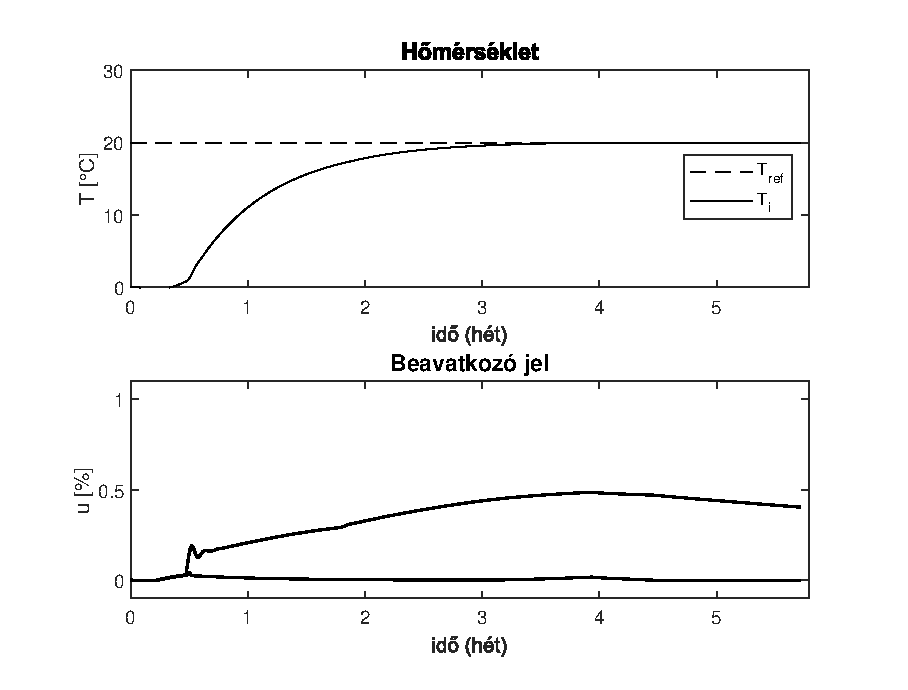
\includegraphics[width=0.8\textwidth]{figures/simscape/mpc}
		\caption{A zárt szabályozási kör ugrásválasza}
		\label{fig:mpc-simulated}
\end{figure}

A fenti ábrán látható a helyesen súlyozott MPC-vel a zárt szabályozási kör viselkedése. Ebben vannak tökéletlenségek, ezekre a fizikai modellnél térek majd rá. A szabályozó paraméterei az alábbi táblázatban láthatók.
\begin{table}[H]
	\footnotesize
	\centering
	%\renewcommand{\arraystretch}{2} % to increase cell height
	%\taburulecolor{gray}
	%\begin{tabular}{|p{0.8cm}|p{1cm}|p{1cm}|p{1cm}|p{1cm}|p{1cm}|p{1cm}|p{1cm}|}
	%
	%\begin{tabulary}{\linewidth}{LLc}
	\begin{tabu}{@{}cl@{}}
		\hline
		$T_s$ 	& 1800 s
		\\ 
		p 		& 50 minta (25 óra)
		\\ 
		c 		& 1
		\\
		$w_u$ 	& 0.005 
		\\ 
		$w_{\Delta u}$ 	& 50
		\\ 
		$w_y$ 	& 20
		\\
		SF 		& 30 
		\\   \hline
	\end{tabu}
	\label{tab:MPCfactors}
	\caption{MPC szabályozó paraméterei}
	%
	%\label{tab:TabularExample}
	%\tabref{TabularExample}~táblázat
\end{table}

\subsection{Fejlesztési lehetőségek a szabályozással kapcsolatban}
	
Épületautomatikai rendszerek használatával, például az iContrALL intelligens otthon rendszerével a fellépő zavarásokat (emberek jelenléte, napsütés, szél) mérhetjük. A szabályozás a zavarások hatásmechanizmusának ismeretében jobb zavarelnyomást tud elérni, sőt az integrációval további beavatkozók is használhatók (például árnyékolástechnikai eszközök).


%\chapter{Tesztek laborkörülmények között}

\section{A kísérleti rendszer}
Az elméleti eredmények validálásához elkészítettem egy szoba kicsinyített modelljét. Ez egy kartondobozban kapott helyet. A doboz hőtároló képessége elég csekély, ezért extra hőtároló tömegeket helyeztem bele, OSB falapot és egy elektromos kályhából vett samott téglát.
A fűtési teljesítményt halogén izzókkal juttattuk a rendszerbe. Ezek teljesítménye szabályozható, így ez a bemenet lineáris a szelepekkel ellentétben, azaz kétszer nagyobb beavatkozójelre kétszer nagyobb teljesítmény kerül a rendszerbe.
A hőmérsékletet mérjük a dobozban és azon kívül is. Zavarásként a mérőszoba ablakát kinyitjuk, így a doboz környezeti hőmérséklete lecsökken.

\begin{figure}[H]
	\centering
	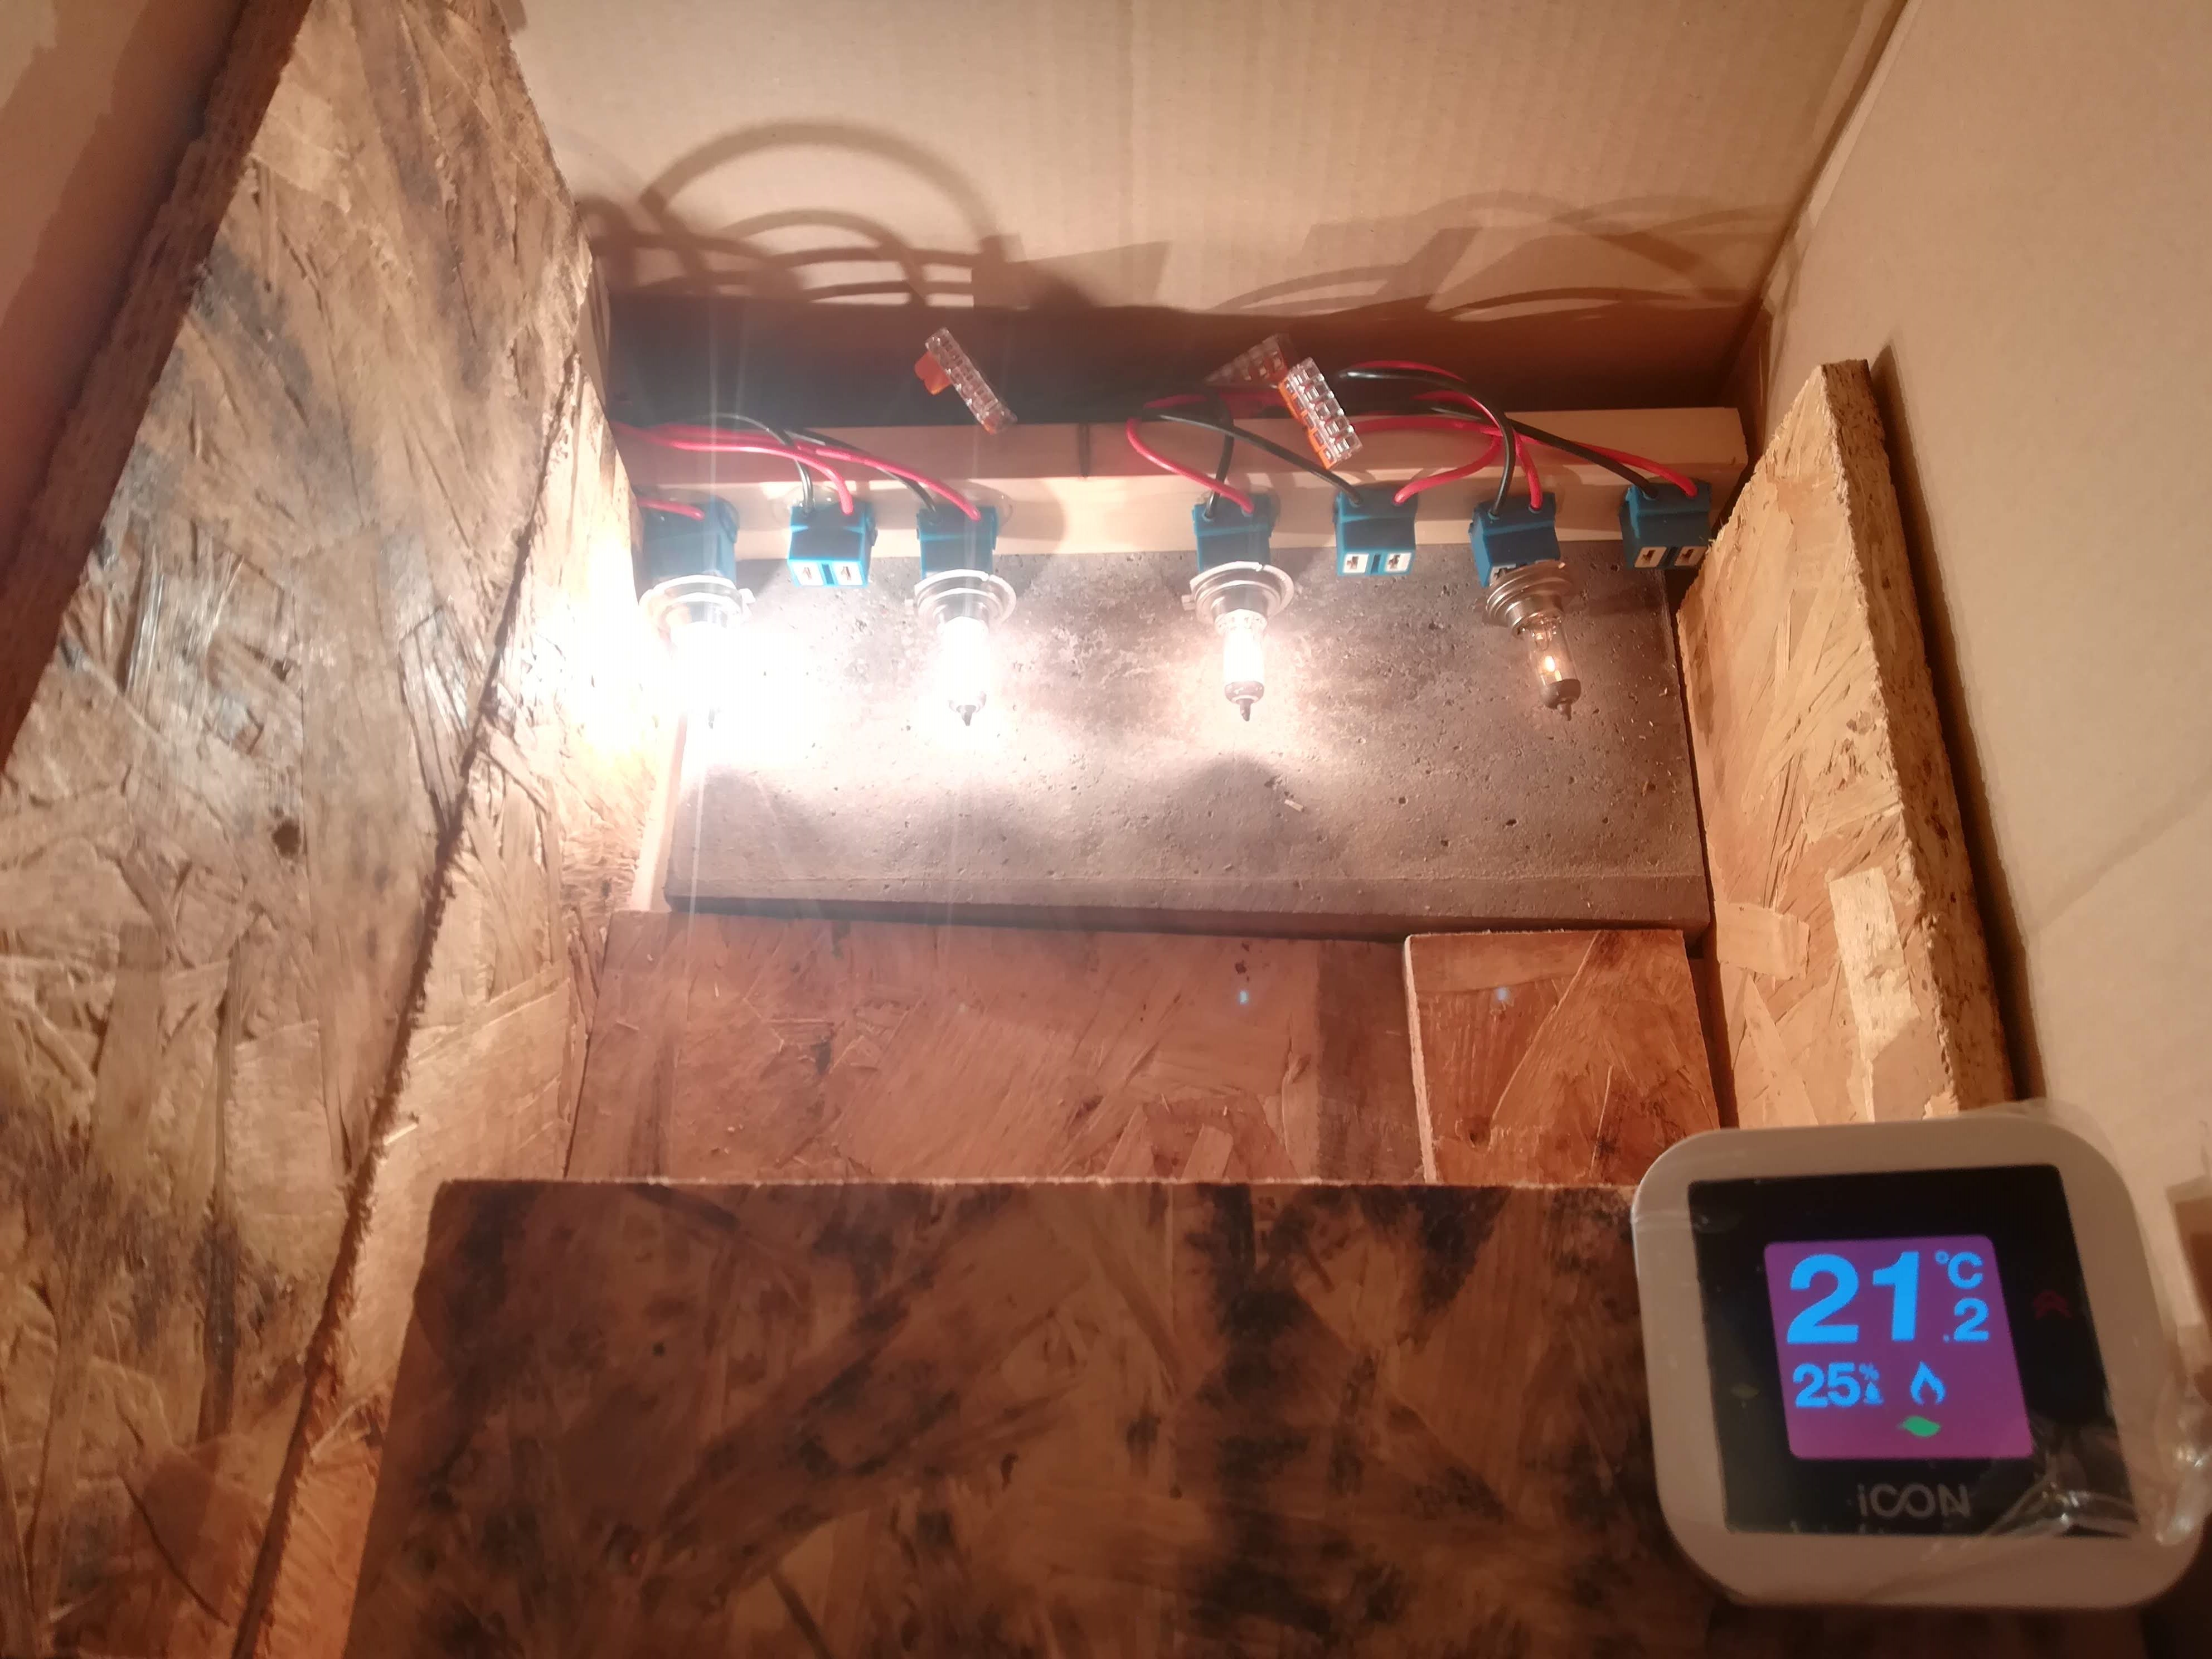
\includegraphics[width=0.8\textwidth]{figures/realsys/interior2}
	\caption{A doboz belseje hőmérővel és szabályozható izzókkal}
	\label{fig:realsys-interior}
\end{figure}

\section{A Simulink konfigurálása}
A valós idejű futáshoz Simulink  Real-time szükséges. A real-time működés itt azt jelenti, hogy a szabályozót a Simulink mintavételi időnként futtatja le. Azaz ha a kísérleti rendszerre \SI{30}{\second}-es mintavételi idejű szabályzót tervezek, akkor az MPC félpercenként mintát fog venni a hőmérsékletekből és ki fog adni egy beavatkozójelet. Így a real-time ez esetben nem jelent például szigorú korlátokat a futásidőre.


%A Real-time UDP-t használom. %https://uk.mathworks.com/help/xpc/io_ref/udp-transport-protocol.html
%https://uk.mathworks.com/products/simulink-desktop-real-time.html

A szabályzó a számítógépen fut, és mintavételi időnként a jelenlegi hőmérsékletet beolvassa, az MPC-t lefuttatja, a beavatkozó jeleket pedig elküldi a beágyazott számítógépnek.

\begin{figure}
	\centering
	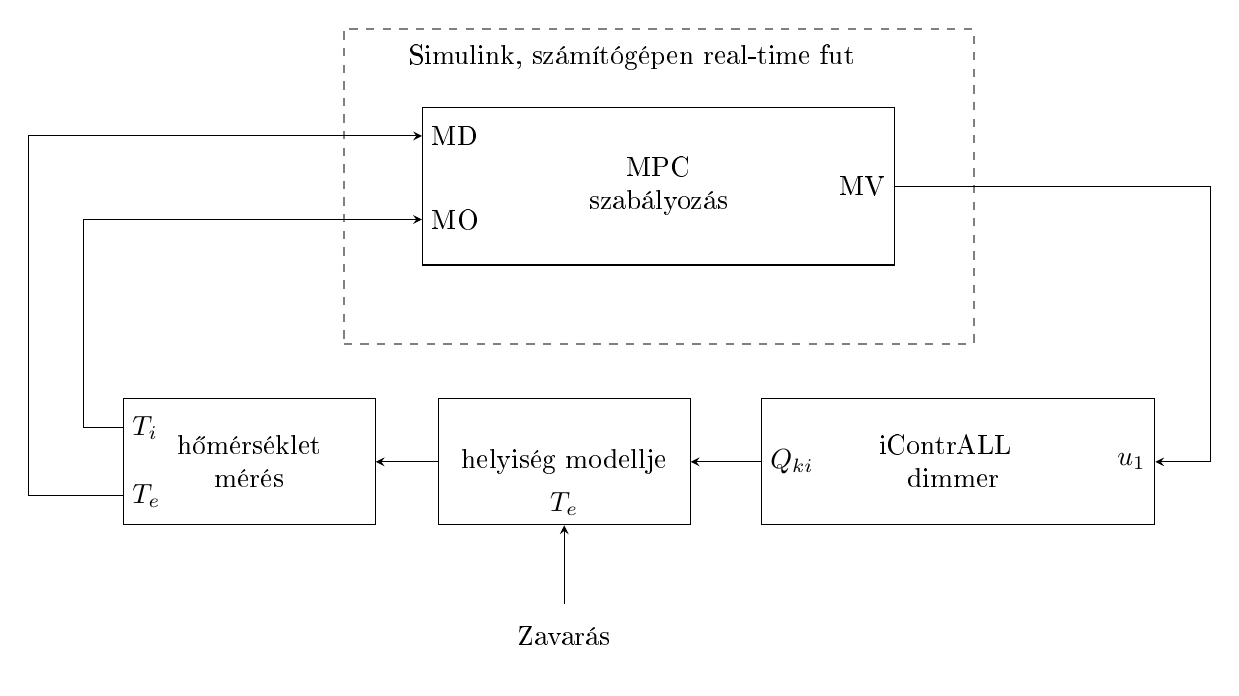
\begin{tikzpicture}[>=stealth,
  		%inner/.style={draw,fill=blue!5,thick,inner sep=3pt,minimum width=8em},
		%outer/.style={draw=gray,dashed,fill=green!1,thick,inner sep=5pt}
		outer/.style={draw=gray,dashed,thick,inner sep=5pt}
		]
	
	% Szabályzási kör elemei
	% ----------------------
	
		% Szabályzó
		\node[draw,rectangle, minimum height=2cm,minimum width=6cm] (MPC) at (3.2,3.5) {\parbox{2cm}{\centering MPC szabályozás}};		

		% Fűtési rendszer
		\node[draw,rectangle, minimum height=1.6cm,minimum width=5cm] (Heat) at (7,0) {\parbox{2cm}{\centering iContrALL~~~~ \\ dimmer~~}};
	
		% Ház
		\node[draw,rectangle, minimum height=1.6cm,minimum width=3.2cm] (House) at (2,0) {helyiség modellje};
		
		% Hőmérő
		\node[draw,rectangle, minimum height=1.6cm,minimum width=3.2cm] (Measure) at (-2,0) {\parbox{2cm}{\centering hőmérséklet\\mérés}};
		
		%Zavarás
		\node[rectangle, minimum height=0.8cm,minimum width=2cm,below=of House, node distance=1cm] (ghostDist)  {Zavarás};

		
	
	% Kiegészítő cuccok
	% ----------------------
	
	% Keret - Matlab
	\node[draw,outer,rectangle, minimum height=4cm,minimum width=8cm,
	label={[label distance=-0.1cm, anchor=north]100:Simulink, számítógépen real-time fut}] (keret) at (3.2,3.5) {};
	
	% Zavarás a modellbemenetre
	\draw[->] (ghostDist.90) --  (House.270) node[above]{$T_e$};
	
	%\draw[->] (ctr.191) node[right]{${u_{2}}$} -| ++(-1.7,1.3)|-  (Numeric.172) node[right]{$\alpha_{floor}$};  %node[above left]{$\alpha_{radiator}$}; 
	
	% mért változók
	\draw[->] (House.180) -- (Measure.0);
	\draw[->] (Measure.195) node[right]{$T_e$} -| ++(-1.2,0)  |-  (MPC.168) node[right]{MD} ;
	\draw[->] (Measure.165) node[right]{${T_{i}}$}-| ++(-0.5,0.8)  |-  (MPC.188) node[right]{MO} ;

	
	%\draw[->] (d.0) node[left]{heat [W]} ->  ++(3,0) ->  (house.180);
	% Beavatkozó jel
	\draw [->] (MPC.0) node[left]{MV} -| ++(4,-2.5)  |- (Heat.0) node[left]{${u_1}$}; %++(1.5cm,0) -- (2cm,0pt) -- (2.5cm,10pt);
	
	\draw[->] (Heat.180)  node[right]{$Q_{ki}$} -- (House.0) ;
	%\draw[->] (d.20) -| ++(1,-1) |- (y.350);
	
	%\path 
	%(d.150)	 edge[<->] 	node[anchor=north,above]{valvePercent}	(y.270);
	
	% Lehetséges label beállítások:
		%label={[blue,yshift=0.3cm]above:Z}]
	
%	\node[draw,outer,rectangle, minimum height=5.5cm,minimum width=13cm,
%	label={[label distance=-0.1cm, anchor=north]270:3 bemenetű, 1 kimenetű szakaszmodell}] (keret) at (0,15) {};
%	
%	
	\end{tikzpicture}

	\caption{A valós idejű mérések szereplői}
	\label{fig:realtimesimulink}
\end{figure}

%\begin{tikzpicture}[>=stealth,remember picture]
%\node[draw,rectangle,inner sep=0.5cm] (y) at (0,0) {$A$};
%\node[draw] (d) at (0,2) {%
%%	\begin{tikzpicture}[remember picture]
%%	\matrix [matrix of math nodes] (mat)
%%	{
%%		B & \phantom{C}   \\
%%		\phantom{B} & C \\
%%	};
%%	\end{tikzpicture}
%%};
%%\draw[->,shorten >= 6pt] (y.west) -| ++(-1,1) |- (mat-1-1);
%%\draw[->,shorten >= 6pt] (y.west) -| ++(-0.8,1) |- (mat-2-1);
%%\draw[->] ($(mat-2-2)+(14pt,0)$) -| ++(0.8,-1) |- (y.east);
%%\draw[->] ($(mat-1-2)+(14pt,0)$) -| ++(1,-1) |- (y.east);
%\end{tikzpicture}




% 3600001117-es ID-jű, Raspberry Pi, IP címe fixen 192.168.0.108, 54321-es port.

%A PI SPI-n küld a rádióadónak.
%Rádiókommunikáció egyirányú.

\section{Szabályozótervezés az identifikált modellre}
Mivel a kísérleti rendszeremnek nincsen energetikai tanúsítványa, identifikáltam az ugrásválaszával (\ref{fig:realsys-ident}. ábra).

\begin{figure}
	\centering
	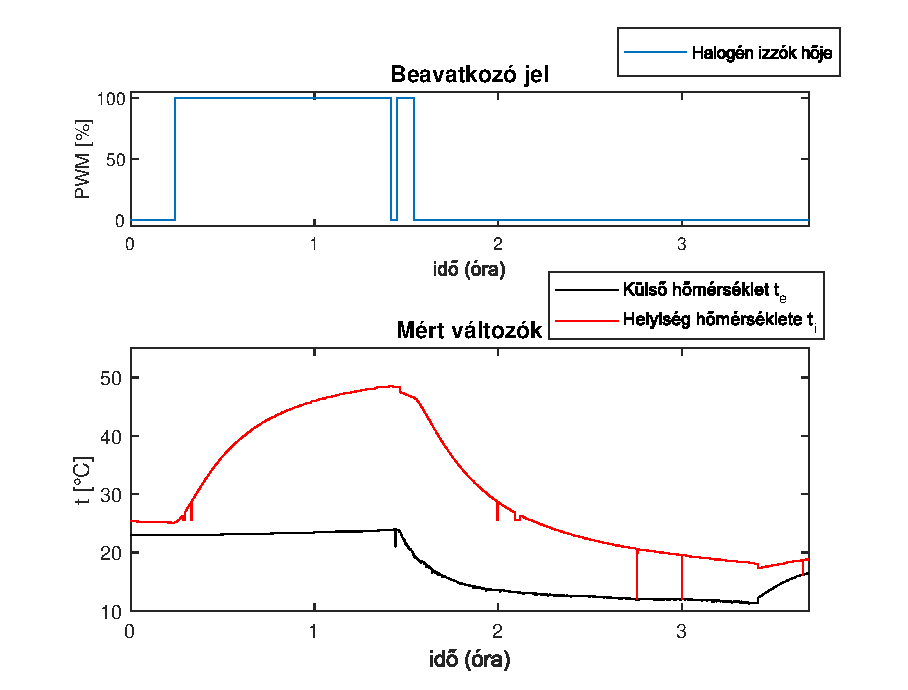
\includegraphics[width=0.65\textwidth]{figures/realsys/ident}
	\caption{Identfikációhoz használt mérési adatsor}
	\label{fig:realsys-ident}
\end{figure}

A valós idejű méréshez használni kívánt szabályozót érdemes először szimulációban megvizsgálni. Ekkor adott a szabályzott szakasz identifikált lineáris modellje, az MPC-t pedig létrehoztam  a modellhez az előző fejezet szerint. Az ott felmerülő nehézségeket, problémákat a fizikai rendszeren szerzett tapasztalatok miatt sikerült megoldani. A Simulinkben a tervezés a \textit{\ref{fig:mpc-sim}. ábra} szerinti elrendezésben történt, használva az MPC szabályozás közbeni (online) hangolásának lehetőségét.



\subsection{Mintavételi idő és predikciós horizont}

Az MPC paraméterezésére \textit{Agachi \cite{romanMPC_Agachi}} könyvében találhatók ajánlások. A predikciós horizontot eszerint úgy kell megválasztani, hogy az a szakasz releváns dinamikáját lefedje. Mivel a felfutási ideje a kísérleti rendszernek körülbelül 1 óra, ezért ezt ekkorára választottam. A predikciós horizont ajánlott nagysága 10-20 mintavétel a számítási igény csökkentése miatt (így $T_s =$ \SI{300}{\second} adódna),  viszont a mérés során gyakrabban szerettem volna látni a változásokat, a mintavételi időt 30 másodpercnek vettem.

\begin{figure}[h]
	\centering
	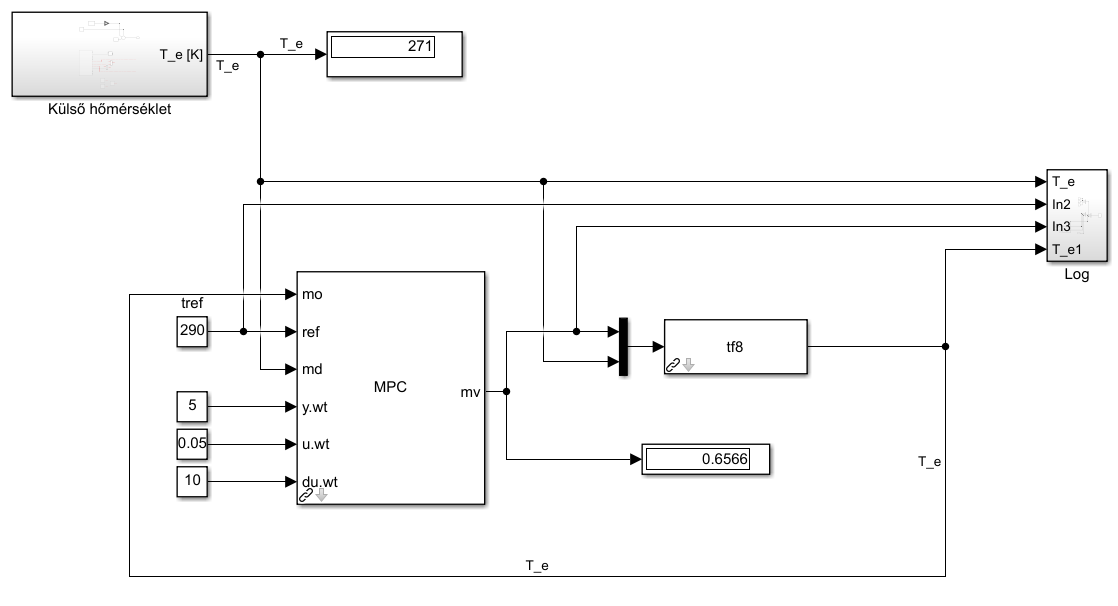
\includegraphics[width=\textwidth]{figures/simscape/simModel}
	\caption{Lineáris modellre MPC szimulációja}
	\label{fig:mpc-sim}
\end{figure}

A fentiek mellett viszont a szabályozó nem adott ki beavatkozójelet egészen egy predikciós horizontnyi ideig, azaz majdnem 1 órán keresztül\footnote{Ha 300 másodperces mintavételi időt használtam és 10 mintányi predikciós horizontot, ugyanez volt a helyzet. Ez idő alatt az MPC valószínűleg az állapotbecslőjét inicializálja.}. Az MPC képes a költségfüggvényben figyelembe venni a predikciós horizonton belül a referenciajel jövőbeli változásait (ez a \textit{Signal Previewing}), ezt kipróbáltam annak érdekében, hogy ezt a \say{holtidőt} csökkentsem, ám ellentétes hatást értem el.

A Simulink blokk viszont támogatja az MPC-nek kezdeti érték megadását. A kezdeti érték nélküli MPC-t szimulációban (azaz nem valós időben) futtattam, majd leolvastam annak belső állapotát. Az \verb|mpcstate| függvénnyel létre kellett hoznom egy objektumot, ami a Simulinkben a szabályzót inicializálja. Ehhez szükség volt a szabályzó állapotteres szakaszmodelljének\footnote{Amikor az MPC-t létrehozzuk, a szakaszmodellt a Matlab állapotteressé alakítja.} becsült állapotára, a zavarjel becsült értékére, a zaj becsült értékére (ez esetben üres vektor), a legutóbbi beavatkozójelre és egy kovarianciamátrixra (ezt nullmátrixnak vettem).

Azzal, hogy a fenti objektumban a legutóbbi beavatkozójelet maximálisnak vettem, valós idejű futás esetén, a fizikai rendszer ugrásválaszánál nem kellett kivárnom egy órát, azaz a predikciós horizontnyi időt, hanem a szabályzó rögtön maximális beavatkozójelet adott ki.

\subsection{A szabályozó költségfüggvénye}

A költségfüggvény súlyait iteratívan választottam ki. A paraméterek akár a szabályozó futása közben is módosíthatók, hatásuk azonnal látható. Először a referenciakövetést leginkább befolyásoló $w_y$ paramétert állítottam be.
 
\begin{figure}[H]
	\centering
	% trim={<left> <lower> <right> <upper>}
	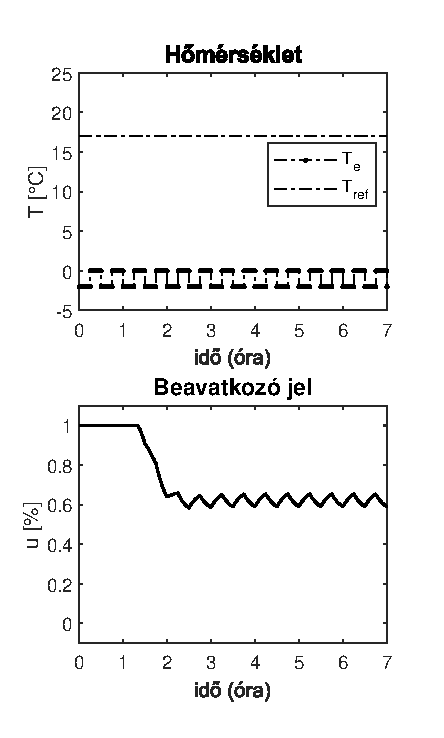
\includegraphics[width=0.4\textwidth, trim=0 168 0 0, clip,]{figures/realsys/disturbpar}
	\caption{Referenciajel és zavarás a szimuláció során}
	\label{fig:mpc-dist}
\end{figure}

\begin{figure}[H]
	\begin{subfigure}[t]{0.32\textwidth}
		\centering
		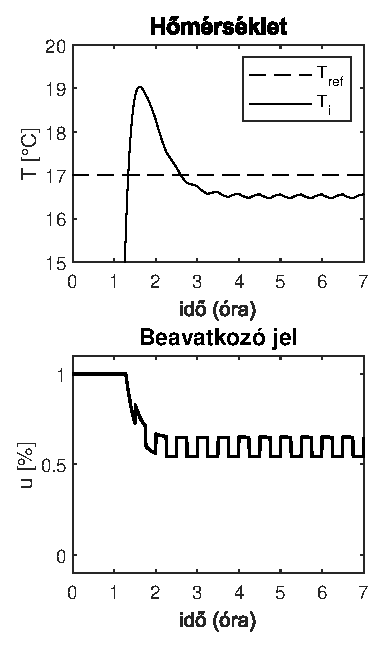
\includegraphics[width=\textwidth]{figures/realsys/mpc-wy-1}
		\caption{$w_y=1$}
		\label{fig:mpc-wy-1}
	\end{subfigure}
	~
	\begin{subfigure}[t]{0.32\textwidth}
		\centering
		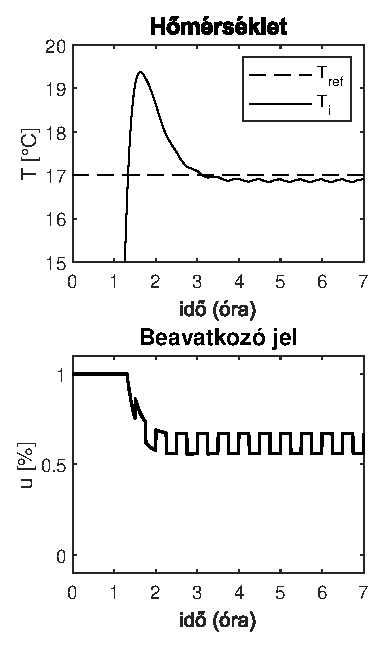
\includegraphics[width=\textwidth]{figures/realsys/mpc-wy-2}
		\caption{$w_y=2$}
		\label{fig:mpc-wy-2}
	\end{subfigure}
	~
	\begin{subfigure}[t]{0.32\textwidth}
		\centering
		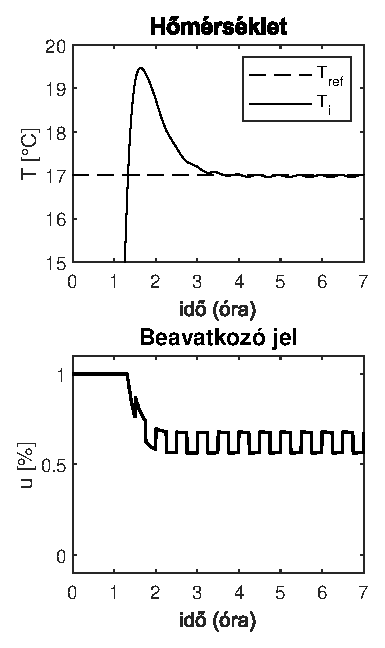
\includegraphics[width=\textwidth]{figures/realsys/mpc-wy-5}
		\caption{$w_y=5$}
		\label{fig:mpc-wy-5}
	\end{subfigure}
	\caption{MPC viselkedése különböző $w_y$ értékekre}
	\label{fig:mpc-wy}
\end{figure}

A \ref{fig:mpc-wy-5}.~ábrán látható esetben volt a legjobb a referenciakövetés, így ezt a paramétert rögzítettem. Következőnek a $w_u$ paraméter értékét választottam meg. Ez a beavatkozójel nagyságát bünteti.

\begin{figure}[H]
\begin{subfigure}[t]{0.32\textwidth}
	\centering
	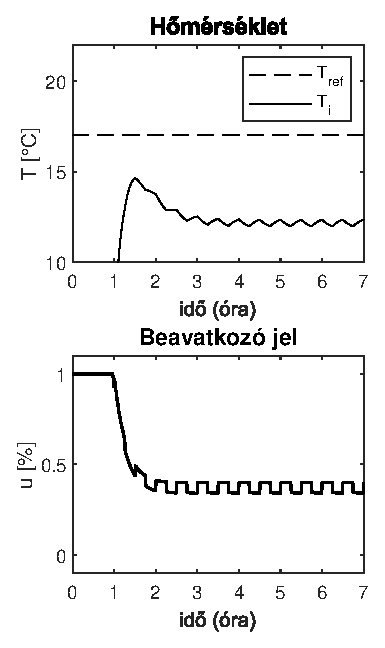
\includegraphics[width=\textwidth]{figures/realsys/mpc-wu-20}
	\caption{$w_u=20$}
	\label{fig:mpc-wu-20}
\end{subfigure}
~
\begin{subfigure}[t]{0.32\textwidth}
	\centering
	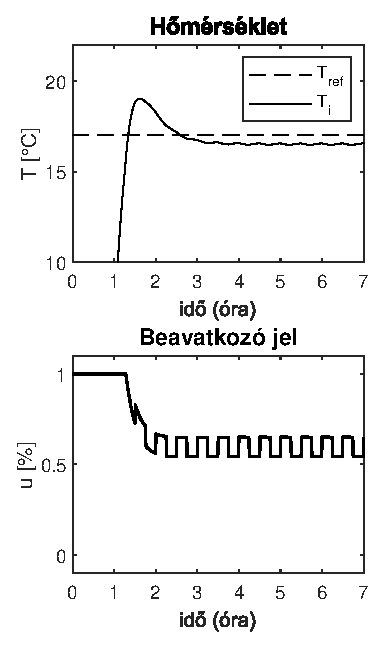
\includegraphics[width=\textwidth]{figures/realsys/mpc-wu-05}
	\caption{$w_u=5$}
	\label{fig:mpc-wu-05}
\end{subfigure}
~
\begin{subfigure}[t]{0.32\textwidth}
	\centering
	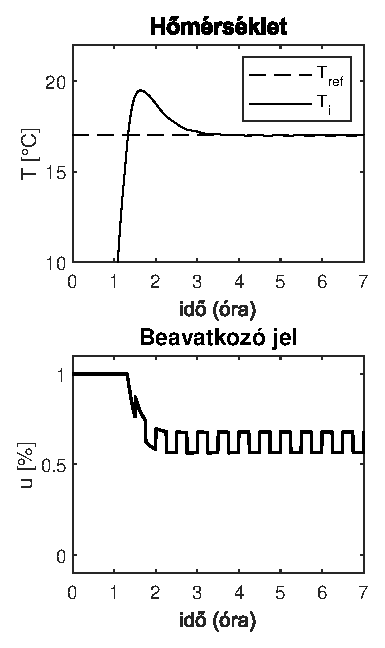
\includegraphics[width=\textwidth]{figures/realsys/mpc-wu-005}
	\caption{$w_u=0.05$}
	\label{fig:mpc-wu-005}
\end{subfigure}
\caption{MPC viselkedése különböző $w_u$ értékekre, $w_y=5$ mellett}
\label{fig:mpc-wu}
\end{figure}
 A \ref{fig:mpc-wu}.~ábrán látható, hogy nagy súly a költségfüggvényben lecsökkent beavatkozójelet, és így nagy követési hibát okoz. A két felsorolt paraméter valójában egymás ellenében hatnak\footnote{Bővebben a paraméterekről: https://uk.mathworks.com/help/mpc/ug/tuning-weights.html}.

A beavatkozást kevésbé büntettem, így a referenciakövetés megmaradt, viszont a túllövés lecsökkent. Most már két fix paraméter mellett választottam súlyt a beavatkozójel változási sebességéhez.

\begin{figure}[H]
\begin{subfigure}[t]{0.32\textwidth}
	\centering
	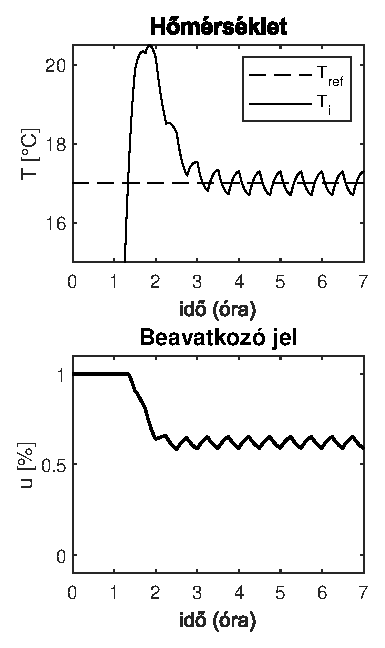
\includegraphics[width=\textwidth]{figures/realsys/mpc-wdu-100}
	\caption{$w_{\Delta u}=100$}
	\label{fig:mpc-wdu-100}
\end{subfigure}
~
\begin{subfigure}[t]{0.32\textwidth}
	\centering
	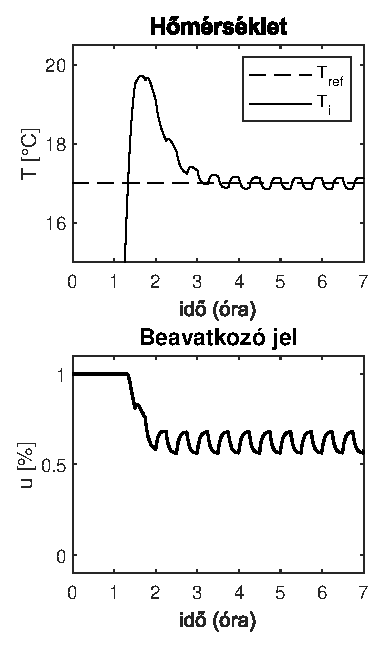
\includegraphics[width=\textwidth]{figures/realsys/mpc-wdu-50}
	\caption{$w_{\Delta u}=50$}
	\label{fig:mpc-wdu-50}
\end{subfigure}
~
\begin{subfigure}[t]{0.32\textwidth}
	\centering
	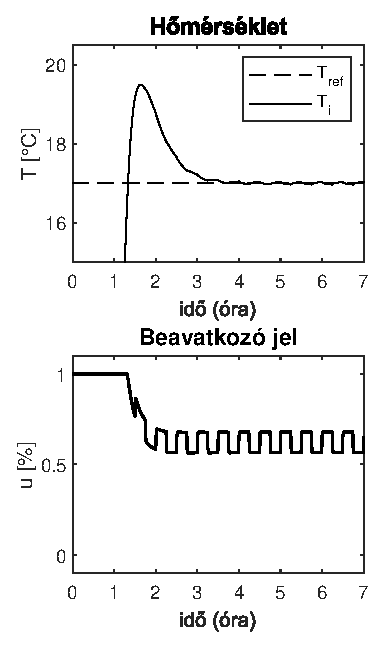
\includegraphics[width=\textwidth]{figures/realsys/mpc-wdu-10}
	\caption{$w_{\Delta u}=10$}
	\label{fig:mpc-wdu-10}
\end{subfigure}
\caption{MPC viselkedése  $w_{\Delta u}$ értékekre, $w_y=5$, $w_u=0.05$ mellett}
\label{fig:mpc-wdu}
\end{figure}

\begin{figure}[H]
	\centering
	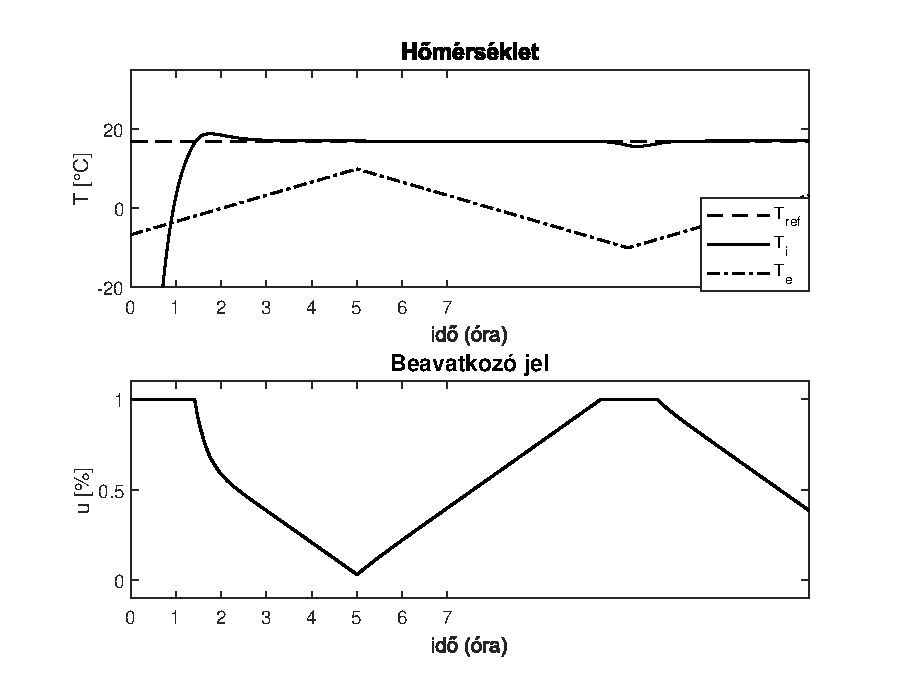
\includegraphics[width=0.7\textwidth]{figures/simscape/distrej}
	\caption{A zárt szabályozási kör ugrásválasza}
	\label{fig:mpc-distrej}
\end{figure}

A \ref{fig:mpc-wdu}. ábrán jól megfigyelhető, hogy nagy súly esetén a beavatkozójel frekvenciája lecsökken\footnote{A beavatkozás alapfrekvenciáját a \textit{\ref{fig:mpc-dist}. ábra} szerinti zavarjel adja, viszont a felfutás sebessége a $w_{\Delta u}$ paramétertől függ.}. Ez az épületgépészeti rendszerekben alacsonyabb energiafelhasználással járhat. Ám a három esetben különböző mértékű lengés tapasztalható állandósult állapotban: ezek közül az igényeknek, illetve a specifikációnak megfelelőt kell kiválasztani. A zavarelnyomást megvizsgáltam nagyobb tartományban változó külső hőmérséklettel is, ez látható a \textit{\ref{fig:mpc-distrej}. ábrán}.

A szabályzót kipróbáltam a kísérleti rendszeren is, a \textit{\ref{fig:realtimesimulink}. ábra} szerinti elrendezésben. A pontozott vonal a doboz környezeti hőmérséklete, a csökkenést az ablak kinyitásával értem el.
A külső hőmérséklet 85 perc környékén \SI{23}{\degreeCelsius}-ról csökkenni kezdett egészen \SI{8}{\degreeCelsius}-ra, de az MPC már a zavarás kezdetekor megnövelte a beavatkozó jelét és tartotta a referencia értéket. 

\begin{figure}[H]
	\centering
	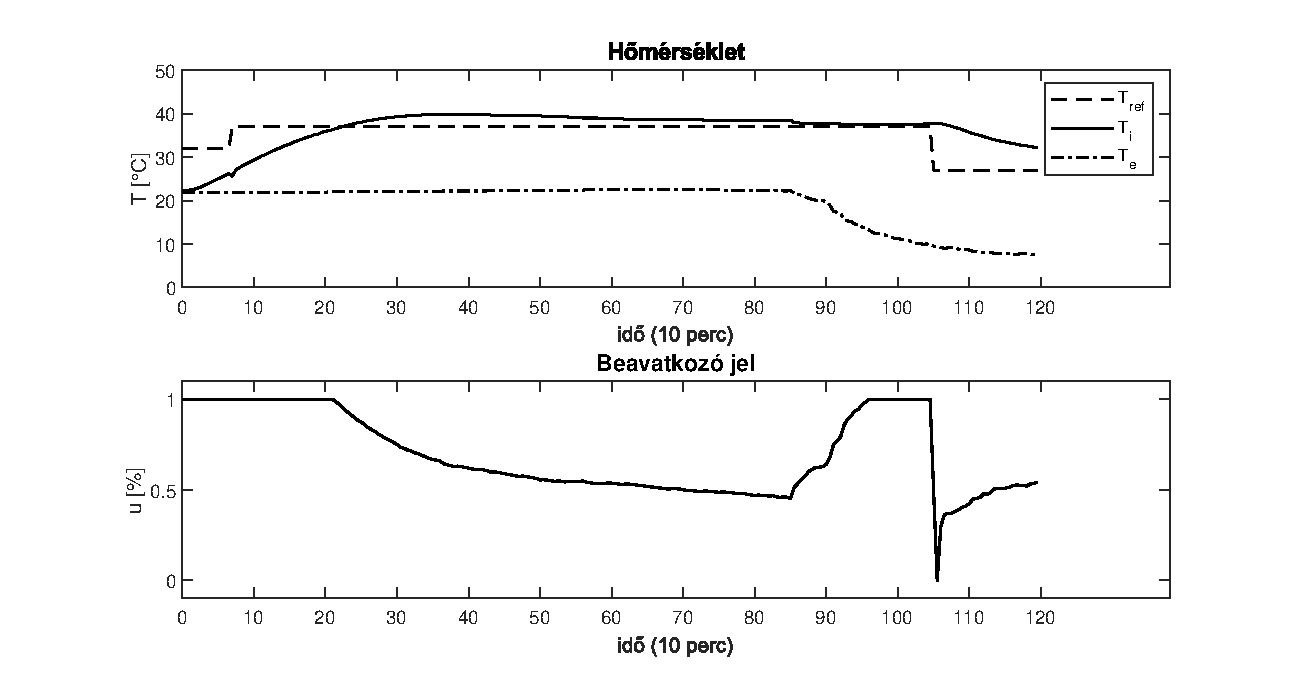
\includegraphics[width=0.95\textwidth]{figures/realsys/step}
	\caption{Mérés a fizikai rendszeren a behangolt MPC-vel}
	\label{fig:mpc-step}
\end{figure}

A tárgyaltakon felül további lehetőségek is vannak a költségfüggvények megadására. \textit{Thieblemont és Schirrer} \cite{SCHIRRER201686} megmutatta, hogy különösen jó eredmény érhető el MPC szabályozás és megújuló energiák kombinált használatával. A költségfüggvényekben például laza megkötéseket is lehet tenni, amik az adott jelet korlátozzák ugyan, de mégis túlléphetők - ilyenek egy napelemes rendszernél könnyen előfordulhatnak. Ekkor a laza felső korlát lehet a napelemes rendszer teljesítménye, de ezen felül is lehet energiát felhasználni a hálózatból.

Szintén \textit{Thieblemont} \cite{THIEBLEMONT2017485} készített felmérést az időjárás-előrejelzéssel kombinált MPC használatáról. (Itt a már korábban említett Signal Prevewing funkció használatos a jövőbeli bemenetek becsléséhez.) Az itt olvasható tapasztalatok és a bemutatott módszerek iránymutatást adhatnak a jövőbeni fejlesztésekhez.


%% Feljesztési lehetőségek
%\begin{formal}
%	Még lehetséges:
%	\begin{itemize}[noitemsep,topsep=-8pt,parsep=0pt,partopsep=0pt]
%		%		\item kazán bekapcsolása
%		%		\item előremenő hőmérséklet - unmeasured VAGY uncontrolled inputként
%		%		\item 1 db. fűtőtest (most radiátor) szelepének tömegárama (szelep áteresztése)
%		%		\item Később több fűtőtest vagy többféle fűtőtestek (padlófűtés, különböző teljesítményű radiátorok) szabályozása
%		\item környezeti hőmérséklet: predikció / szekvencia használata% is lesz rá. Hatása a kimeneten már identifikálva lett, 3 pólussal és 2 zérussal tökéletesen lekövethető.
%		\item napsugárzás zavaró hatása% - szimulálható  a bizonytalansága valószínűleg nagy lesz
%	\end{itemize}
%	
%	Belső változók - fűtési rendszer és ház kapcsolata
%	\begin{itemize}[noitemsep,topsep=-6pt,parsep=0pt,partopsep=0pt]
%		\item napsugárzás - radiatív, az ablak felületével és a szöggel arányos
%		\item fűtőtestek sugárzó és konvektív hőárama
%	\end{itemize}
%	
%	Paraméterek a plantben nem állandók:
%	\begin{itemize}[noitemsep,topsep=-6pt,parsep=0pt,partopsep=0pt]
%		%		\item hőátadási tényezők hőmérsékletfüggők, áramlási sebesség-függők (szél)
%		\item szellőztetés, belső hőterhelés hatása
%	\end{itemize}
%\end{formal}
%\chapter{Összefoglalás}

A félév során egy olyan témakörrel foglalkoztam, amihez szükség volt az alapképzés során szerzett összes rendszer- és irányításelméleti tudásra. Kellő hálózatelméleti szemlélettel az épületfizikai összefüggéseket szinte egy betűcserével be lehetett fogadni, hiszen a jelenségek analógok az elektromos hálózatokkal.

Számos tapasztalattal lettem gazdagabb a szabályozásokkal kapcsolatban is, a kutatómunka során rengeteg forrást áttekintettem. A tématerületbe való betekintés motivációt ad a mesterképzés tárgyaihoz is, mivel már ismerem az ilyen típusú szabályozók egyes gyakorlati alkalmazásait.


\chapter*{Köszönetnyilvánítás}
Köszönöm a segítséget és a motivációt konzulenseimnek, szüleimnek, munkatársaimnak. Az épületbejárás szervezéséért köszönet a BME Építész Klubnak.


\pagebreak
\bibliographystyle{unsrt}
\bibliography{szakdogaforras}

%\bibliography{szakdogaforras}
%%\addcontentsline{toc}{chapter}{Irodalomjegyzék}
%\bibliographystyle{plain}

%\include{appendices}

\label{page:last}
\end{document}
